\documentclass[preprint,12pt,authoryear]{elsarticle}
\usepackage[letterpaper,hmargin=0.9in,top=0.76in,bottom=0.78in]{geometry}
\usepackage[T1]{fontenc}
\usepackage{lmodern,textcomp}
\usepackage{xcolor}
\usepackage{booktabs,tabularx,array}
\usepackage{float}
\usepackage{listings}
\usepackage{tikz}
\usepackage{tcolorbox}
\usepackage[hidelinks]{hyperref}

% ============================================================
% References to the main paper: edit here if its numbering changes
% ============================================================
\newcommand{\papertitle}{A Neuro-Symbolic Architecture for Safe and Feasible Self-Recovery in Multi-Agent Manufacturing Systems}
\newcommand{\FigOutline}{Fig.~5}
\newcommand{\FigComposition}{Fig.~6}

% ============================================================
% Page and heading style (as in the template)
% ============================================================
\pagestyle{plain}
\setlength{\parindent}{0pt}
\setlength{\parskip}{3pt}
\raggedbottom
\setlength{\intextsep}{7pt plus 2pt minus 2pt}
\setlength{\abovecaptionskip}{4pt}
\setlength{\belowcaptionskip}{0pt}
\makeatletter
\renewcommand\section{\@startsection{section}{1}{\z@}%
  {14pt plus 4pt minus 2pt}{6pt plus 2pt minus 2pt}{\large\bfseries\boldmath}}
\renewcommand\subsection{\@startsection{subsection}{2}{\z@}%
  {9pt plus 3pt minus 2pt}{2pt plus 1pt minus 1pt}{\normalsize\bfseries}}
\makeatother

% ============================================================
% Colours: the paper's own (blue LLM and Product Agent, green RA, purple CCA)
% ============================================================
\definecolor{pablue}{RGB}{31,99,171}
\definecolor{ragreen}{RGB}{56,118,29}
\definecolor{ccapurple}{RGB}{112,48,160}
\definecolor{refred}{RGB}{192,0,0}
\definecolor{cutgray}{gray}{0.45}

% ============================================================
% Recorded text: set verbatim, wrapped at spaces with a small indent, no wrap symbol
% ============================================================
\lstdefinestyle{record}{
  basicstyle=\fontsize{9}{11}\selectfont\ttfamily,
  columns=fullflexible, keepspaces=true, showstringspaces=false, upquote=true,
  breaklines=true, breakatwhitespace=true, breakindent=9.5pt, breakautoindent=true,
  prebreak={}, postbreak={},
  aboveskip=0pt, belowskip=0pt,
  escapeinside={(*@}{@*)}
}
\lstset{style=record}
\lstdefinestyle{quoteline}{style=record, xleftmargin=1.2em, aboveskip=2pt, belowskip=4pt}

% A cut inside a recorded line, and recorded lines left out.
\newcommand{\cut}{{\normalfont\ttfamily\color{cutgray}[...]}}
\newcommand{\vd}{\raisebox{-0.1ex}{\vbox{\baselineskip 3pt\lineskip 0pt\lineskiplimit 0pt\hbox{.}\hbox{.}\hbox{.}}}}
\newcommand{\skipped}[1]{{\normalfont\color{cutgray}\vd\enspace{\itshape\footnotesize #1}}}
% Who wrote the lines that follow (our label, not recorded text).
\newcommand{\who}[2]{{\normalfont\sffamily\bfseries\footnotesize\color{#1}#2}}
% A bar in the margin beside the line to notice.
\newcommand{\notebar}[1]{\rlap{\hspace{-5pt}\textcolor{#1}{\rule[-0.35ex]{2pt}{1.9ex}}}}
% Recorded text inside a table cell.
\newcommand{\rec}[1]{{\ttfamily\frenchspacing #1}}

% Identifiers in running text.
\urlstyle{tt}
\let\code\nolinkurl

% Verdict marks, drawn so that they look the same in every engine.
\newcommand{\ok}{\tikz[baseline=-0.55ex]{\draw[line width=0.9pt, color=ragreen!80!black, line cap=round, line join=round] (0,0) -- (0.08,-0.09) -- (0.24,0.12);}}
\newcommand{\no}{\tikz[baseline=-0.55ex]{\draw[line width=0.9pt, color=refred, line cap=round] (0,-0.09) -- (0.19,0.11) (0,0.11) -- (0.19,-0.09);}}
\newcommand{\na}{\textcolor{cutgray}{--}}

% ============================================================
% Gray titled box (as in the template); never breaks across a page
% ============================================================
\newtcolorbox{recbox}[1]{colback=black!2, colframe=gray!60, arc=4pt, boxrule=0.4pt,
  left=7pt, right=7pt, top=5pt, bottom=5pt, fonttitle=\small\bfseries, title={#1},
  before skip=2pt, after skip=3pt}

\newcolumntype{Y}{>{\raggedright\arraybackslash}X}

\begin{document}

\begin{center}
  {\Large\bfseries \papertitle\par}
  \medskip
  {\large Supplementary Material\par}
\end{center}

This supplement follows one recovery from the experiments, Part slippage, from the failure to
robot motion. Appendix~A shows how the recovery outline was synthesized one event at a time,
each proposal checked by the Resource Agent (RA) and the Central Controller Agent (CCA)
(\FigOutline{} of the paper). Appendix~B shows how one accepted event was composed from robot
primitives (\FigComposition). Appendix~C reports the execution of the composed programs in
Gazebo. The run uses the neuro-symbolic framework at the event level, with Claude Opus~5.5 at
medium reasoning effort.\footnote{The run was recorded before the correction of the Exit model
described in the paper. None of its events uses Exit.}

In the gray boxes, monospaced text is copied from the records of this run. A gray
\cut{} marks a cut inside a line, and a gray dotted line marks lines left out. Replies are
JSON; their line breaks and indentation are ours. Every prompt and reply of the run is in the
supplementary files, in the folder \code{transcripts/part_slippage/} (\code{outline.md} and
\code{composition.md}).

\appendix
\makeatletter
\@addtoreset{table}{section}
\@addtoreset{figure}{section}
\makeatother
\renewcommand{\theHtable}{\Alph{section}.\arabic{table}}
\renewcommand{\theHfigure}{\Alph{section}.\arabic{figure}}

% ============================================================
\section{Recovery Outline Synthesis}\label{sec:outline}
% ============================================================

\subsection{The failure}

During normal production, robot \code{ur5e-4} was carrying the small gear to the assembly
board and lost it on the way. It stopped above the board and reports a fault. The gear came to
rest on the table, at no station. Robot \code{ur5e-3} was waiting at the buffer with the square
peg in its gripper. Figure~\ref{fig:scene} shows the scene.

A recovery therefore has to free the gripper of \code{ur5e-3}, move \code{ur5e-4} away from the
board, pick up the gear and place it. The large language model (LLM) is given the measurements,
not these conclusions.

\begin{figure}[H]
\centering
\begin{minipage}[c]{0.47\linewidth}
\centering
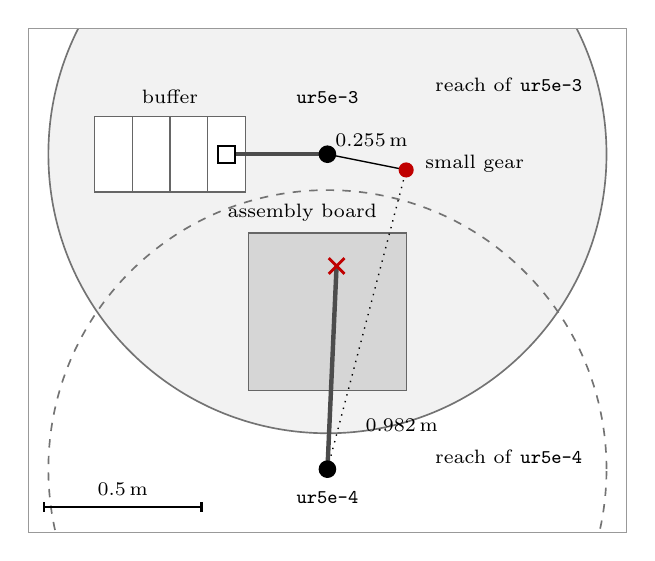
\begin{tikzpicture}[x=4.0cm,y=4.0cm,font=\scriptsize]
  \begin{scope}
    \clip (-0.95,-0.70) rectangle (0.95,0.90);
    % reach of ur5e-3 (solid, shaded) and of ur5e-4 (dashed)
    \fill[black!5] (0,0.5) circle [radius=0.886];
    \draw[black!55, line width=0.6pt] (0,0.5) circle [radius=0.886];
    \draw[black!55, line width=0.6pt, dashed] (0,-0.5) circle [radius=0.886];
    % assembly board area and the four buffer zones
    \fill[black!16] (-0.25,-0.25) rectangle (0.25,0.25);
    \draw[black!60] (-0.25,-0.25) rectangle (0.25,0.25);
    \fill[white] (-0.74,0.38) rectangle (-0.26,0.62);
    \draw[black!60] (-0.74,0.38) rectangle (-0.26,0.62);
    \draw[black!60] (-0.62,0.38) -- (-0.62,0.62) (-0.50,0.38) -- (-0.50,0.62) (-0.38,0.38) -- (-0.38,0.62);
  \end{scope}
  \draw[black!40] (-0.95,-0.70) rectangle (0.95,0.90);
  % the two distances to the gear
  \draw[black, line width=0.5pt] (0,0.5) -- (0.25,0.45);
  \draw[black, line width=0.5pt, dotted] (0,-0.5) -- (0.25,0.45);
  % arms, from base to gripper
  \draw[line width=1.6pt, black!70] (0,0.5) -- (-0.32,0.5);
  \draw[line width=1.6pt, black!70] (0,-0.5) -- (0.029,0.145);
  \fill (0,0.5) circle [radius=0.028];
  \fill (0,-0.5) circle [radius=0.028];
  % gripper of ur5e-3 with the square peg; gripper of ur5e-4 over the gear's slot
  \filldraw[fill=white, draw=black, line width=0.6pt] (-0.347,0.473) rectangle (-0.293,0.527);
  \draw[refred, line width=1pt] (0.004,0.120) -- (0.054,0.170) (0.004,0.170) -- (0.054,0.120);
  % the fallen gear
  \fill[refred] (0.25,0.45) circle [radius=0.024];
  % labels
  \node[anchor=south] at (0,0.63) {\texttt{ur5e-3}};
  \node[anchor=north] at (0,-0.54) {\texttt{ur5e-4}};
  \node[anchor=south] at (-0.50,0.63) {buffer};
  \node[anchor=south] at (-0.08,0.255) {assembly board};
  \node[anchor=west] at (0.28,0.47) {small gear};
  \node[anchor=south] at (0.14,0.495) {0.255\,m};
  \node[anchor=west] at (0.09,-0.36) {0.982\,m};
  \node[anchor=east] at (0.84,0.72) {reach of \texttt{ur5e-3}};
  \node[anchor=east] at (0.84,-0.46) {reach of \texttt{ur5e-4}};
  % scale bar
  \draw[line width=0.8pt] (-0.90,-0.62) -- (-0.40,-0.62);
  \draw[line width=0.8pt] (-0.90,-0.635) -- (-0.90,-0.605) (-0.40,-0.635) -- (-0.40,-0.605);
  \node[anchor=south] at (-0.65,-0.615) {0.5\,m};
\end{tikzpicture}
\end{minipage}\hfill
\begin{minipage}[c]{0.50\linewidth}
\footnotesize\raggedright
The small gear (red dot) lies on the table at (0.250, 0.450), outside the board area and at
no station.\par\smallskip
It is 0.255\,m from the base of \code{ur5e-3} and 0.982\,m from the base of \code{ur5e-4}.
Each arm reaches 0.886\,m, so only \code{ur5e-3} can pick it up.\par\smallskip
The gripper of \code{ur5e-3} (white square) holds the square peg, above zone~4 of the
buffer.\par\smallskip
The gripper of \code{ur5e-4} (red cross) stopped over the gear's slot. \code{ur5e-4} is
inside the board area, where only one robot may be at a time.
\end{minipage}
\caption{The cell at the failure, seen from above and drawn to scale from the recorded positions.}
\label{fig:scene}
\end{figure}

Table~\ref{tab:names} lists the names that appear in the records and what they mean in the paper.

\begin{table}[H]
\centering\footnotesize
\setlength{\tabcolsep}{5pt}
\begin{tabularx}{\linewidth}{@{}>{\raggedright\arraybackslash}p{5.9cm} Y@{}}
\toprule
In the records & Meaning \\
\midrule
\code{candidate_events}; \code{c1}, \code{c2} & The recovery events the LLM proposes in one turn, in its order of preference. The event names and these labels are the LLM's. \\
\code{RECOVERY_SEQ1} to \code{RECOVERY_SEQ4} & The accepted recovery events $e^R_1$ to $e^R_4$. From turn~4 on, the LLM numbers its own candidates this way. \\
\code{expected_end_state} & The intended end state of an event: the values it promises for its robot and its part. \\
\code{FEASIBLE}, \code{INFEASIBLE}; \code{SAFE}, \code{UNSAFE} & Verdicts of the RA's feasibility validation and of the CCA's safety validation. \\
\code{recovery_complete}; \code{NONBLOCKING} & The LLM declares the recovery complete; the CCA's verdict that production can still be completed. \\
\code{primitive_steps}; \code{context_ref} & The program of primitives for one event; a reference to a value that the RA holds or calculates. \\
\code{gear_small}, \code{KET4_Square_4mm}, \code{assembly_board-v1} & The small gear, the square peg, the assembly board. \\
\bottomrule
\end{tabularx}
\caption{Names used in the records.}\label{tab:names}
\end{table}

\subsection{What the LLM is given}

Table~\ref{tab:prompt} is the first prompt of the run with five of its seven sections folded.
The Failure and Recovery Goal sections are printed in full. They hold measurements and one
target condition for the small gear. They do not say which robot should fetch the gear, that
\code{ur5e-3} must first put down the square peg, or that \code{ur5e-4} must leave the board.

\begin{table}[H]
\begin{recbox}{Outline prompt, turn 1 (user message)}
% begin recorded prompt-t1
\begin{lstlisting}
(*@\skipped{Task and Role: 3 lines; its instruction is quoted below}@*)
Failure
What was detected and measured, stated the same way for every resource.
- ur5e-4 did not complete place_approach of gear_small (destination_location assembly_board-v1)
- task_outcome (ur5e-4, task environment_9): goal_cancelled true, terminal_status 5, progress 0.503
- device_fault_report (ur5e-4): resource_state failed, reported_by gripper object detection
- state_discrepancy (ur5e-4, gear_small): expected_holder ur5e-4, measured_holder null
- gear_small: not held, not at any station, measured at (0.250, 0.450, 1.025)
- ur5e-4: measured pose (0.029, 0.145, 1.289), inside assembly_board-v1

Recovery Goal
- gear_small: part_location assembly_board-v1 (target Gear_Plate/Gear_Shaft_1) (normally ur5e-4's place_insert; ur5e-4 failed)
(*@\skipped{Candidate Rules: 7 rules on how to write one recovery event}@*)
(*@\skipped{Knowledge Base: 11 references the LLM may ask for}@*)
(*@\skipped{Resources: 12 lines, one per resource, with its recorded state and declared capabilities}@*)
(*@\skipped{Parts: 12 lines, one per part, with its location and assembly target}@*)
\end{lstlisting}
% end recorded prompt-t1
\end{recbox}
\caption{The first prompt of the run. Two sections are complete; five are folded.}\label{tab:prompt}
\end{table}

The folded sections hold the rules for writing an event and the recorded state and declared
capabilities of every resource and part. In full, the prompt is about 17,500 characters, nearly
two thirds of it the Resources section. None of the seven prompts of this run has a section of
safety rules. The instruction that sets up the loop of \FigOutline{} is in Task and Role:

% begin recorded prompt-t1-instruction
\begin{lstlisting}[style=quoteline]
(*@\cut@*) Propose 2(*@\textendash@*)5 different ways to do the next step of that plan, most preferred first. The first one in your order that passes every check becomes the next recovery event; the others are dropped.
\end{lstlisting}
% end recorded prompt-t1-instruction

\subsection{The run, turn by turn}

In each turn the LLM asks the knowledge base for facts (\code{need_context}), proposes two to
five candidate events in its order of preference, or declares the recovery complete
(\code{recovery_complete}). The RA checks the candidates in that order for feasibility, and the
CCA checks each feasible one for safety. The first candidate that passes both checks becomes the
next recovery event; the candidates after it are not checked. Table~\ref{tab:ledger} is the
whole run. Twice a refusal went back to the LLM, and both times the next proposal changed.

\begin{table}[H]
\centering\footnotesize
\setlength{\tabcolsep}{4pt}
\begin{tabularx}{\linewidth}{@{}c Y l l l@{}}
\toprule
Turn & LLM reply & \textcolor{ragreen}{RA feasibility} & \textcolor{ccapurple}{CCA safety} & Result \\
\midrule
1 & Asks for 8 facts; the first is \code{/parts/gear_small/pose_relations} & \na & \na & facts added \\
\addlinespace[2pt]
2 & \code{place_KET4_on_assembly_board} (\code{ur5e-3}) & \ok\ \code{FEASIBLE} & \no\ \code{UNSAFE} & refused \\
 & \multicolumn{4}{@{}p{\dimexpr\linewidth-1.1cm\relax}@{}}{\raggedright\textcolor{ccapurple}{\bfseries Reason from the CCA:} \rec{SAFE\_shared\_area\_mutex (At most one resource may occupy the assembly\_board-v1 destination area at any time.) is broken during the event: ur5e-3 is in assembly\_board-v1 while ur5e-4 is in assembly\_board-v1}} \\
2 & \code{stage_KET4_in_buffer} (\code{ur5e-3}) & \ok\ \code{FEASIBLE} & \ok\ \code{SAFE} & event 1 \\
\addlinespace[2pt]
3 & \code{retract_ur5e4_home_clear_board} (\code{ur5e-4}) & \ok\ \code{FEASIBLE} & \ok\ \code{SAFE} & event 2 \\
\addlinespace[2pt]
4 & \code{pick_dropped_gear_small_ur5e3} (\code{ur5e-3}), stating a pose & \no\ \code{INFEASIBLE} & \na & refused \\
4 & \code{pick_dropped_gear_small_ur5e3_grip_center} (\code{ur5e-3}), stating a pose & \no\ \code{INFEASIBLE} & \na & refused \\
 & \multicolumn{4}{@{}p{\dimexpr\linewidth-1.1cm\relax}@{}}{\raggedright\textcolor{ragreen}{\bfseries Reason from the RA:} \rec{gear\_small's recorded position gives ur5e-3's target, so this event takes no pose; it states \{x: 0.250, y: 0.450, z: 1.243\}}} \\
\addlinespace[2pt]
5 & \code{pick_dropped_gear_small_ur5e3} (\code{ur5e-3}), no pose & \ok\ \code{FEASIBLE} & \ok\ \code{SAFE} & event 3 \\
\addlinespace[2pt]
6 & \code{place_gear_small_on_board_ur5e3} (\code{ur5e-3}) & \ok\ \code{FEASIBLE} & \ok\ \code{SAFE} & event 4 \\
\addlinespace[2pt]
7 & Declares the recovery complete & \na & \ok\ \code{NONBLOCKING} & outline accepted \\
\bottomrule
\end{tabularx}
\caption{Outline synthesis for Part slippage: 7 turns, 8 facts looked up, 68,402 tokens, 4 accepted events.}\label{tab:ledger}
\end{table}

A dash means the check was not run. Turns 2 to 6 proposed 3, 2, 2, 2 and 2 candidates; one
ranked after the accepted candidate was not checked and is not listed.

\subsection{Two refusals and what the LLM did next}

Table~\ref{tab:cca} follows the first refusal through three consecutive records. In turn~2 the
LLM's first choice was to let \code{ur5e-3} place the square peg on the board. The RA found it
feasible. The CCA refused it, because \code{ur5e-4} was still in the board area. The next prompt
carried the reason, and the next plan begins by sending \code{ur5e-4} home. This reason is the
first place where the LLM reads the name of a safety rule.


The second candidate of turn~2, staging the peg in the buffer, passed both checks and became
event~1. Sending \code{ur5e-4} home became event~2.

The RA refused once as well. In turn~4 the LLM proposed to pick up the gear and wrote a position
for the arm into the end state. The Candidate Rules of the prompt say when a position may be
stated:

% begin recorded prompt-t1-pose-rule
\begin{lstlisting}[style=quoteline]
(*@\cut@*) Give `pose` only for a position nothing else gives: an arm's pick or place target comes from the part or the place when it declares compute_pick_targets or compute_place_targets, (*@\cut@*)
\end{lstlisting}
% end recorded prompt-t1-pose-rule

Table~\ref{tab:ra} shows the end state before and after the refusal. The pose was refused for
being stated, not for being wrong: the height in the second candidate, 1.253\,m, is the one the
RA itself calculates later (\ref{sec:composition}).


\begin{table}[H]
\begin{recbox}{Outline, turns 2 and 3: refused by the CCA, then revised}
% begin recorded cca-refusal
\begin{lstlisting}
(*@\who{pablue}{LLM reply, turn 2: its first candidate}@*)
"event_name": "place_KET4_on_assembly_board",
(*@\skipped{resource ur5e-3, part and end state}@*)
"rationale": "ur5e-3 reaches assembly_board-v1 and already has this placement as its pending task, so completing it frees the gripper without wasted work."
(*@\who{ccapurple}{Prompt, turn 3: the section added after the refusal}@*)
Validation Feedback
These candidates were refused, and stage_KET4_in_buffer, listed after them, was applied.
- candidate_event=c1/ur5e-3/KET4_Square_4mm | event_name=place_KET4_on_assembly_board | constraint_code=cca_safety | reason=SAFE_shared_area_mutex (At most one resource may occupy the assembly_board-v1 destination area at any time.) is broken during the event: ur5e-3 is in assembly_board-v1 while ur5e-4 is in assembly_board-v1
(*@\who{pablue}{LLM reply, turn 3}@*)
"plan": "ur5e-4 is failed and still occupies the assembly_board-v1 area, which blocks ur5e-3, so first clear it by sending ur5e-4 home. Then ur5e-3, whose envelope contains gear_small, picks the gear and inserts it at Gear_Plate/Gear_Shaft_1 on assembly_board-v1.",
\end{lstlisting}
% end recorded cca-refusal
\end{recbox}
\caption{A safety refusal, the feedback in the next prompt, and the next reply.}\label{tab:cca}
\end{table}

\begin{table}[H]
\begin{recbox}{Event 3, picking up the gear: refused in turn 4, accepted in turn 5}
% begin recorded ra-refusal
\begin{minipage}[t]{0.485\linewidth}
\begin{lstlisting}
(*@\who{pablue}{LLM reply, turn 4, first candidate}@*)
"expected_end_state": {
  "held_part": "gear_small",
  "resource_state": "picked",
  "resource_location": null,
(*@\notebar{refred}@*)  "pose": {"x": 0.25, "y": 0.45, "z": 1.243},
  "part_location": "ur5e-3"
},
\end{lstlisting}
\end{minipage}\hfill
\begin{minipage}[t]{0.485\linewidth}
\begin{lstlisting}
(*@\who{pablue}{LLM reply, turn 5, first candidate}@*)
"expected_end_state": {
  "resource_state": "picked",
  "held_part": "gear_small",
  "resource_location": null,
  "part_location": "ur5e-3"
},
\end{lstlisting}
\end{minipage}

\vspace{3pt}{\color{gray!60}\hrule height 0.3pt}\vspace{3pt}
\begin{lstlisting}
(*@\who{ragreen}{Between the two, in the prompt of turn 5: the section added after the refusal}@*)
Validation Feedback
- candidate_event=RECOVERY_SEQ3/ur5e-3/gear_small | event_name=pick_dropped_gear_small_ur5e3 | constraint_code=ra_feasibility | reason=gear_small's recorded position gives ur5e-3's target, so this event takes no pose; it states {x: 0.250, y: 0.450, z: 1.243}
(*@\skipped{one more line: the same reason for the second candidate}@*)
\end{lstlisting}
% end recorded ra-refusal
\end{recbox}
\caption{A feasibility refusal: the end state before and after, and the feedback between them.}\label{tab:ra}
\end{table}

\subsection{The accepted outline}

Table~\ref{tab:outline} lists the four accepted events, the recovery outline
$s^R = e^R_1 e^R_2 e^R_3 e^R_4$. In turn~7 the LLM declared the recovery complete. The CCA then
checked that the outline is nonblocking: it explored 368 states of its model, starting from the
state the four events leave, and found that normal production can still be completed. The
outline was accepted. In the table, a \code{resource_location} of \code{null} means the robot
is at no named station, and a held part is located at its holder.

\begin{table}[H]
\centering\footnotesize
\setlength{\tabcolsep}{5pt}
\begin{tabularx}{\linewidth}{@{}c l l Y@{}}
\toprule
Event & Name given by the LLM & Resource & Intended end state (\code{resource_state} first) \\
\midrule
1 & \code{stage_KET4_in_buffer} & \code{ur5e-3} & \code{placed}; \code{held_part} \code{null}; the square peg is in \code{zone_1} of the buffer \\
2 & \code{retract_ur5e4_home_clear_board} & \code{ur5e-4} & \code{idle}; \code{resource_location} \code{home} \\
3 & \code{pick_dropped_gear_small_ur5e3} & \code{ur5e-3} & \code{picked}; \code{held_part} \code{gear_small}; \code{resource_location} \code{null}; \code{part_location} \code{ur5e-3} \\
4 & \code{place_gear_small_on_board_ur5e3} & \code{ur5e-3} & \code{placed}; \code{held_part} \code{null}; the gear is at \code{assembly_board-v1}, its assembly at \code{Gear_Plate/Gear_Shaft_1} completed \\
\bottomrule
\end{tabularx}
\caption{The accepted recovery outline.}\label{tab:outline}
\end{table}

\subsection{The other settings}

The experiments in the paper compare this setting with three others. Each changes the prompt in
one place; their prompts are not reproduced here.

% begin recorded other-settings
\begin{lstlisting}[style=quoteline]
(*@\who{black}{Baseline and Informed baseline, event level: no checks during synthesis}@*)
(*@\cut@*) The first one becomes the next recovery event; the others are dropped.
(*@\who{black}{Informed baseline: also adds a section, Safety Rules, that lists the seven safety rules}@*)
(*@\who{black}{Outline level, all three methods: the whole outline in one reply}@*)
(*@\cut@*) Give the whole plan in `events`: every recovery event, in the order they happen.
\end{lstlisting}
% end recorded other-settings

% ============================================================
\section{Primitive Composition of Event 3}\label{sec:composition}
% ============================================================

Appendix~B follows event~3, picking up the dropped gear. \FigComposition{} of the paper sketches
the same event. For each accepted event the RA prompts the LLM again, now for a program of the
robot's primitives. The prompt holds the event with its start and end states, the names of the
eight primitives and five predefined functions of \code{ur5e-3}, and fifteen references through
which everything else must be requested. One line of its Output Contract shapes every program:

% begin recorded comp-contract
\begin{lstlisting}[style=quoteline]
- Each step MUST include params. Every number in params is a {"context_ref": ...}; strings and booleans may be literals from served context.
\end{lstlisting}
% end recorded comp-contract

So the LLM writes no coordinates. A \code{context_ref} names a value that the RA holds or
calculates.

Composing event~3 took three calls. In call~5 the LLM submitted nothing and asked for eleven
facts: the contracts of five primitives, the predefined functions \code{pick_approach} and
\code{pick_grasp}, the state and model of \code{ur5e-3} at the start of the event, and the
gear's state and recorded pose. In call~6 it submitted a program that passed the gear's pose
into \code{compute_pick_targets}, and the RA's check returned one finding
(Table~\ref{tab:revision}). In call~7 it submitted the program in Table~\ref{tab:program},
whose first step passes only the part name, and the RA accepted it.

\FigComposition{} of the paper draws the first four steps; the fifth withdraws the arm with the
gear. The arm stops 0.228\,m above the gear's measured height, because its recorded pose is that
of its controlled link, which lies above its fingertips. In Table~\ref{tab:revision},
\code{recovery-resource-3@localhost} is the address of the agent of \code{ur5e-3},
\code{composition_missing_context} is the check's code for the finding, and the owner in the
rationale is the resource whose primitive it is, here \code{ur5e-3}.

\begin{table}[H]
\centering\footnotesize
\setlength{\tabcolsep}{5pt}
\begin{tabularx}{\linewidth}{@{}c l Y Y@{}}
\toprule
Step & Primitive & Written by the LLM & Resolved by the RA \\
\midrule
1 & \code{compute_pick_targets} & the part name & the approach, target and retreat poses, calculated from the gear's recorded position \\
2 & \code{move_cartesian} & a reference to the approach pose & (0.250, 0.450, 1.303) \\
3 & \code{move_cartesian} & a reference to the target pose & (0.250, 0.450, 1.253) \\
4 & \code{grasp_part} & the part name; its model name by reference & \code{gear_small}; the gear is then held \\
5 & \code{move_cartesian} & a reference to the retreat pose & (0.250, 0.450, 1.303) \\
\bottomrule
\end{tabularx}
\caption{The accepted program for event 3. Positions are in metres.}\label{tab:program}
\end{table}

\begin{table}[H]
\begin{recbox}{Composition of event 3, calls 6 and 7: the finding and the revision}
% begin recorded comp-revision
\begin{lstlisting}
(*@\who{pablue}{LLM reply, call 6: the parameters of step 1, compute\_pick\_targets}@*)
"part_name": "gear_small",
"target_pose": {
  "x": {"context_ref": "/parts/gear_small/observed_pose/x"},
(*@\skipped{y, z and model\_name, written the same way}@*)
},
"target_pose_source": "observed_pose"
(*@\who{ragreen}{Prompt, call 7: the section added after the RA's check}@*)
Previous Validation Feedback (read first)
- RECOVERY_SEQ3 / recovery-resource-3@localhost [composition_missing_context]: compute_pick_targets: target_pose (*@\cut@*) differs from None, the input the composition's calculation reads; compute_pick_targets: target_pose_source 'observed_pose' differs from '', the input the composition's calculation reads
(*@\who{pablue}{LLM reply, call 7}@*)
"rationale": "Following the validation finding, compute_pick_targets no longer receives target_pose or target_pose_source, so the owner calculation reads the recorded pose itself.",
(*@\skipped{the accepted program: step 1, and the first parameter of step 2}@*)
{"primitive": "compute_pick_targets", "params": {"part_name": "gear_small"}},
"x": {"context_ref": "event_facts.pick_targets.gear_small.approach_pose.x"},
\end{lstlisting}
% end recorded comp-revision
\end{recbox}
\caption{The one revision in the composition of event 3.}\label{tab:revision}
\end{table}

The RA then checked the five steps against its model of \code{ur5e-3} without moving the robot,
resolved every reference to a value (Table~\ref{tab:program}) and recorded
\code{FEASIBLE}: the program leaves the end state that the event promised. The two programs
write references in two ways, with slashes in call~6 and dots in call~7; both are accepted.
Composing all four events took 9 LLM calls and 144,642 tokens: calls 1 and 2 for event~1, 3 and
4 for event~2, 5 to 7 for event~3, and 8 and 9 for event~4.

% ============================================================
\section{Execution in Gazebo}\label{sec:gazebo}
% ============================================================

The four composed programs were then run in Gazebo, starting from the reproduced failure. All
four events completed (Table~\ref{tab:gazebo}).

\begin{table}[H]
\centering\footnotesize
\setlength{\tabcolsep}{5pt}
\begin{tabularx}{\linewidth}{@{}c l Y c >{\raggedright\arraybackslash}p{5.4cm}@{}}
\toprule
Event & Resource & Primitive steps, in order & Calls & What happened in Gazebo \\
\midrule
1 & \code{ur5e-3} & \code{compute_place_targets}, \code{move_cartesian} twice, \code{release_part}, \code{move_cartesian} & 2 & Released the square peg in zone~1 of the buffer. \\
2 & \code{ur5e-4} & \code{move_to_named_pose} & 2 & Moved to its \code{home} pose. \\
3 & \code{ur5e-3} & \code{compute_pick_targets}, \code{move_cartesian} twice, \code{grasp_part}, \code{move_cartesian} & 3 & Moved to the heights 1.303\,m and 1.253\,m over the gear and grasped it. \\
4 & \code{ur5e-3} & \code{compute_place_targets}, \code{move_cartesian} twice, \code{release_part}, \code{move_cartesian} & 2 & Released the gear at its slot on the assembly board. \\
\bottomrule
\end{tabularx}
\caption{The four composed programs as run in Gazebo.}\label{tab:gazebo}
\end{table}

The feasibility and safety checks of Appendices~A and~B were made before this run. The run
replays the composed programs and does not repeat those checks. Every motion uses the values
resolved during composition. The calculation steps are repeated in the simulation for comparison
only; in event~1 the repeated calculation did not resolve the placement geometry of the buffer.
The run ends when the fourth event completes.

In total, the outline took 7 LLM turns and 68,402 tokens, and the composition 9 LLM calls and
144,642 tokens. In the supplementary files:

{\footnotesize\raggedright
\textbf{Video}\enspace \code{videos/part_slippage/recovery_20x.mp4}\par
\textbf{Every prompt and reply}\enspace \code{transcripts/part_slippage/outline.md} and
\code{transcripts/part_slippage/composition.md}\par
\textbf{Raw records}\enspace \code{records/part_slippage/outline/} and
\code{records/part_slippage/composition/}\par}

\end{document}
